\documentclass[11pt]{amsart}
\usepackage[dvipsnames]{xcolor}
\usepackage[utf8]{inputenc}
\usepackage{amssymb,amsmath,amsthm,amsfonts,fullpage,float,latexsym,bbm,microtype,cite,fancyvrb, cite, verbatim, parskip}
\usepackage{tikz}
\usetikzlibrary{decorations.pathreplacing}
\usetikzlibrary{graphs,graphs.standard,calc}
\usepackage[colorinlistoftodos]{todonotes}

\begin{document}

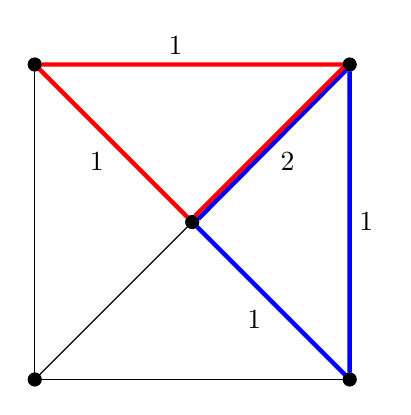
\begin{tikzpicture}[scale=1]

% Vertices
\node[fill,circle,draw, scale=0.5] (v1) at (2,2) {};
\node[fill,circle,draw, scale=0.5] (v2) at (2,-2) {};
\node[fill,circle,draw, scale=0.5] (v3) at (-2,-2) {};
\node[fill,circle,draw, scale=0.5] (v4) at (-2,2) {};
\node[fill,circle,draw, scale=0.5] (C) at (0,0) {};

% Edges (Square outer cycle)
\draw (v1) -- (v2) -- (v3) -- (v4) -- (v1);

\draw (v3) -- (C);

% Edges from v1 to C (red and blue)
\draw[blue, ultra thick] (v1.237) -- (C.27);
\draw[red,  ultra thick] (v1.205) -- (C.65); % Adjust angles for red edge

% Colored edges for cycles
\draw[blue, ultra thick] (v1) -- (v2) -- (C);
\draw[red, ultra thick] (v1) -- (v4) -- (C);


%labelling edges
\path (C) -- node[midway, below right ] {2} (v1);
\path (C) -- node[midway, below left ] {1} (v4);
\path (v1) -- node[midway, above left ] {1} (v4);
\path (C) -- node[midway, below left ] {1} (v2);
\path (v1) -- node[midway, right ] {1} (v2);



\end{tikzpicture}

\end{document}